\section{CMOS Technologie\skript{Kap. 3}}
\subsection{Chipherstellung}
\begin{minipage}{10cm}
	\begin{enumerate}[nosep, noitemsep]
	  \item \textbf{Oberflächenbeschichtung} \\
	  	Epitaxie, Oxidation oder Abscheideverfahren
	  \item \textbf{Fotolithografie} \\
	  	Auftragen von Fotolack, anschliessend belichten (maskieren)
	  \item \textbf{Ätzen} \\
	  	Abtragen der Beschichtung \\
	  	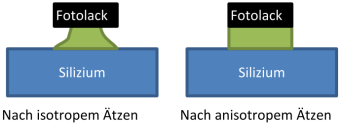
\includegraphics[width=4cm]{images/Aetzen_Isotrop_Anisotrop.png}
	  \item \textbf{Dotieren} \\
	  	Anschluss der Schicht erstellen
	  \item \textbf{Säubern der Wafer}
	\end{enumerate}
\end{minipage}
\begin{minipage}{8cm}
	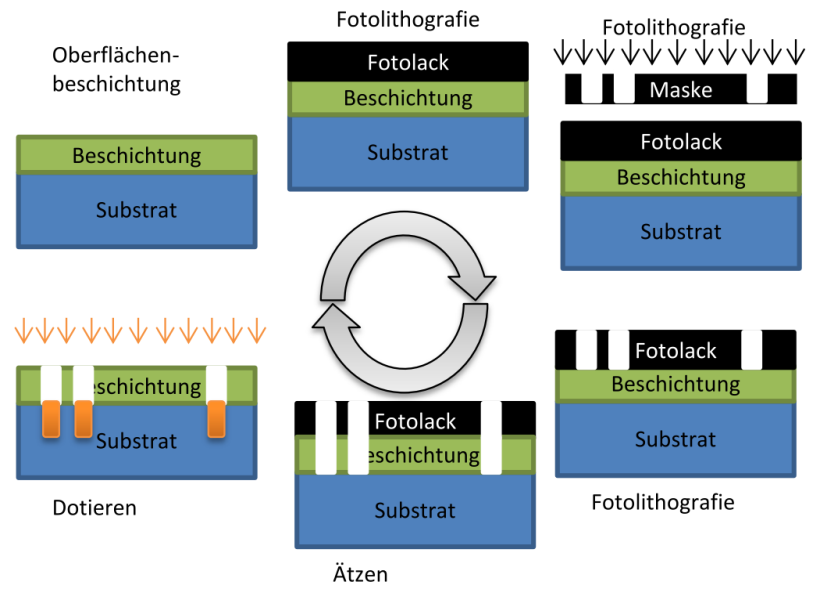
\includegraphics[width=8cm]{images/Chip_Herstellung.png}
\end{minipage}
